\documentclass[12pt, a4paper, UTF8]{ctexart}
\pagestyle{plain}
\usepackage[a4paper, margin=1.25in]{geometry}
\usepackage{xcolor}
\usepackage{listings}
\setmonofont{Monaco}[AutoFakeBold]
\lstnewenvironment{cpplist}{
  \lstset{
    language=C++,
    basicstyle=\footnotesize\ttfamily\zihao{5},
    keywordstyle=\color{purple}\bfseries\zihao{5},
    commentstyle=\color{gray},
    frame=lines,
    tabsize=2,
    lineskip=-1.5pt,
    extendedchars=true,
    escapeinside=``,
    breaklines=true,
    showspaces=false,
    showstringspaces=false,
    showtabs=false,
    }
}{}
\newcommand{\cppinput}[1]{
  \lstinputlisting[
    language=C++,
    basicstyle=\footnotesize\ttfamily\zihao{5},
    keywordstyle=\color{purple}\bfseries\zihao{5},
    commentstyle=\color{gray},
    frame=lines,
    tabsize=2,
    lineskip=-1.5pt,
    extendedchars=true,
    escapeinside=``,
    breaklines=true,
    showspaces=false,
    showstringspaces=false,
    showtabs=false,
  ]{#1}
}
\usepackage[colorlinks=true]{hyperref}
\usepackage{tikz}
\usepackage{graphicx}
\usepackage{caption}
\usepackage{makeidx}
\makeindex

\title{2022蓝桥杯 B组省赛 题解}
\author{Kenshin2438}
\date{\today}

\begin{document}
\maketitle
\tableofcontents
\newpage

\section*{前言}
题目地址: \url{http://oj.daimayuan.top/course/18/problems}

代码仅供参考(已通过上述OJ测试)

\section{九进制转十进制}
简单做一个进制转换即可,
\[
  2 \times 9^3 + 0 \times 9^2 + 2 \times 9^1 + 2 \times 9^0 = 1478
\]
% \cppinput{A.cpp}

\section{顺子日期}
官方的\textbf{顺子}未定义,存在歧义。按照代码源上的注释,应当是14天。分别为,
\[
2022/01/2* \quad 2022/10/12 \quad 2022/11/23 \quad 2022/12/3*
\]
% \cppinput{B.cpp}

\section{刷题统计}
一周一共能做 $5a+2b$ 题,容易知道需要的整周数目。除却整周的部分,最后一周里判断是在前5天还是后2天做完即可。
\cppinput{C.cpp}

\section{修剪灌木}
先简单模拟一下过程:每棵灌木,被修剪时有两种可能——从左往右和从右往左。那么,实际上就有两种可能的高度$2\times(n-i)$和$2\times(i-1)$。
\cppinput{D.cpp}

\section{X进制减法}
由于题目保证 $A \geq B$ ,那么自然是每个数位上的进制越小,两者的差值越小。注意细节:\emph{最小的进制为2进制}。
\cppinput{E.cpp}

\section{统计子矩阵}
枚举子矩形的上下两侧的位置,不妨令子矩阵夹在第 $i,j$ 行之间。然后则需要统计,有多少对不同的 $l,r (l \leq r)$ 使得子矩阵位于 $l,r$ 列之间的时候总和小于 $k$ ,显然这个问题被压缩到了一维——如下图,等价为找到满足求和不大于 $k$ 的不同连续区间的个数。

\begin{center}
  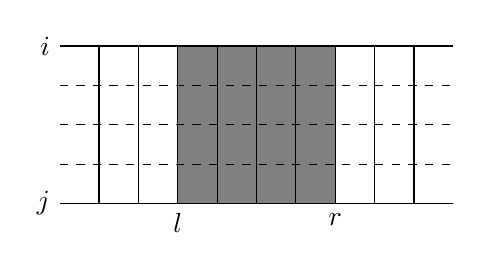
\begin{tikzpicture}
    \node[left] (A) at (0, 0) {$j$};
    \node[left] (B) at (0, 2) {$i$};
    \draw (A) -- (5, 0);
    \draw (B) -- (5, 2);
    \filldraw[fill = gray]
      (1.5, 0) node[below] {$l$} -- (3.5, 0) node[below] {$r$} -- (3.5, 2) -- (1.5, 2) -- (1.5, 0) -- cycle;
    \foreach \i in {0.5, 1.0, ..., 4.0}
      {\draw (\i, 0) rectangle (\i + 0.5, 2);}
    \foreach \i in {0.5, 1.0, 1.5}
      {\draw[dashed] (0, \i) -- (5, \i);}
  \end{tikzpicture}
\end{center}

枚举 $i,j$ 两行的时间复杂度为 $\mathcal{O}(n^2)$ ,如果此时再枚举 $l,r$ 则在时间复杂度上 $\mathcal{O}(n^2m^2)$ 无法通过(仍可拿下 70\% 的分)。该问题是\textbf{滑动窗口}的经典题,最后一步仅需要 $\mathcal{O}(m)$ 即可,详细实现见代码,练习可以去\href{https://leetcode.cn/}{LeetCode}。
\cppinput{F.cpp}

\section{积木画}
很明显,本题用到的算法为\textbf{动态规划}。由于使用的方块最多只能影响到2列,假设当前处理到第 $i$ 列,并且前 $i-2$ 列均被覆盖,则第 $i-1$ 列上的方块有4中可能的状态。

\begin{figure}[htbp]
  \centering
  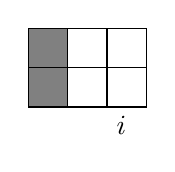
\begin{tikzpicture}
    {
      \filldraw[fill = gray] (0, 0) rectangle (0.5, 0.5); 
      \draw (0.5, 0) rectangle (1, 0.5);
      \draw (1, 0) rectangle (1.5, 0.5);
    }
    {
      \filldraw[fill = gray] (0, 0.5) rectangle (0.5, 1);
      \draw (0.5, 0.5) rectangle (1, 1);
      \draw (1, 0.5) rectangle (1.5, 1);
    }
    \node[below right] (A) at (1, 0) {$i$};
  \end{tikzpicture}
  \qquad
  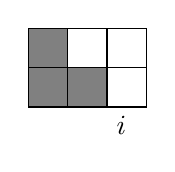
\begin{tikzpicture}
    {
      \filldraw[fill = gray] (0, 0) rectangle (0.5, 0.5); 
      \filldraw[fill = gray] (0.5, 0) rectangle (1, 0.5);
      \draw (1, 0) rectangle (1.5, 0.5);
    }
    {
      \filldraw[fill = gray] (0, 0.5) rectangle (0.5, 1);
      \draw (0.5, 0.5) rectangle (1, 1);
      \draw (1, 0.5) rectangle (1.5, 1);
    }
    \node[below right] (A) at (1, 0) {$i$};
  \end{tikzpicture}
  \qquad
  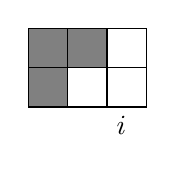
\begin{tikzpicture}
    {
      \filldraw[fill = gray] (0, 0) rectangle (0.5, 0.5); 
      \draw (0.5, 0) rectangle (1, 0.5);
      \draw (1, 0) rectangle (1.5, 0.5);
    }
    {
      \filldraw[fill = gray] (0, 0.5) rectangle (0.5, 1);
      \filldraw[fill = gray] (0.5, 0.5) rectangle (1, 1);
      \draw (1, 0.5) rectangle (1.5, 1);
    }
    \node[below right] (A) at (1, 0) {$i$};
  \end{tikzpicture}
  \qquad
  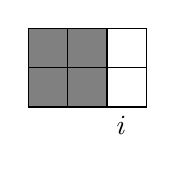
\begin{tikzpicture}
    {
      \filldraw[fill = gray] (0, 0) rectangle (0.5, 0.5); 
      \filldraw[fill = gray] (0.5, 0) rectangle (1, 0.5);
      \draw (1, 0) rectangle (1.5, 0.5);
    }
    {
      \filldraw[fill = gray] (0, 0.5) rectangle (0.5, 1);
      \filldraw[fill = gray] (0.5, 0.5) rectangle (1, 1);
      \draw (1, 0.5) rectangle (1.5, 1);
    }
    \node[below right] (A) at (1, 0) {$i$};
  \end{tikzpicture}
\end{figure}

上述四种状态,从左至右分别定义为 $0, 1, 2, 3$,以\texttt{dp[i][s]}表示处理完前$i$列且状态为$s$的方案数。则可知答案为 \texttt{dp[n][3]} 。
\cppinput{G.cpp}

\section{扫雷}
由于爆炸半径均不超过$10$,可以直接建图,此时的边数目为$\mathcal{O}(nR^2)$,其后使用 BFS 或者 DFS 遍历即可。同时,由于坐标范围比较大,这里需要Hash来储存(代码使用 \texttt{std::unordered\_map} 实现,常数较大)。
\cppinput{H.cpp}

\section{李白打酒加强版}

显然也是\textbf{动态规划}统计方案数,但本题的状态很多(剩余的酒的数目)。容易知道,酒的数目一定要小于等于剩下的花的数目,这样才能满足最终把酒喝完,以此可以排除许多的非法状态。

以\texttt{dp[i][j][k]}表示已经遇到了$i$次店,$j$次花,当前还有$k$斗酒的方案数。那么最终答案就为\texttt{dp[n][m-1][1]}。
\cppinput{I.cpp}

\section{砍竹子}
容易发现,操作 $H \rightarrow \lfloor\sqrt{\lfloor\frac{H}{2}\rfloor+1}\rfloor$ 会使得 $H$ 快速收敛至 $1$ 。我们以这样一种思路来考虑:

假设已经砍了 $i-1$ 棵竹子,当前是第 $i$ 颗。首先,当前的竹子一定会经过上述的操作到达 $1$ 。这个过程中可能会出现 \emph{当前竹子的高度与前一颗竹子在某一时刻的高度一致} 的情况,一旦出现则表明此后的步骤可以同前一颗竹子一起进行。使用二分、\texttt{std::set}或\texttt{std::map}等均可通过此题。
\cppinput{J.cpp}

\end{document}